%%%%%%%%%%%%%%%%%%%%%%%%%%%%%%%%%%%%%%%%%%%%%%%%%%%%%%%%%%%%%%%%%%%%%%%%%%%%%%%%
\documentclass[twocolumn]{revtex4}

%%%%%%%%%%%%%%%%%%%%%%%%%%%%%%%%%%%%%%%%%%%%%%%%%%%%%%%%%%%%%%%%%%%%%%%%%%%%%%%%
% Note that comments begin with a "%" and are not turned into text in the .pdf
% document.
%%%%%%%%%%%%%%%%%%%%%%%%%%%%%%%%%%%%%%%%%%%%%%%%%%%%%%%%%%%%%%%%%%%%%%%%%%%%%%%%

%%%%%%%%%%%%%%%%%%%%%%%%%%%%%%%%%%%%%%%%%%%%%%%%%%%%%%%%%%%%%%%%%%%%%%%%%%%%%%%%
% Include some extra packages.
%%%%%%%%%%%%%%%%%%%%%%%%%%%%%%%%%%%%%%%%%%%%%%%%%%%%%%%%%%%%%%%%%%%%%%%%%%%%%%%%
\usepackage[]{graphicx}
%%%%%%%%%%%%%%%%%%%%%%%%%%%%%%%%%%%%%%%%%%%%%%%%%%%%%%%%%%%%%%%%%%%%%%%%%%%%%%%%

%%%%%%%%%%%%%%%%%%%%%%%%%%%%%%%%%%%%%%%%%%%%%%%%%%%%%%%%%%%%%%%%%%%%%%%%%%%%%%%%
\begin{document}

%%%%%%%%%%%%%%%%%%%%%%%%%%%%%%%%%%%%%%%%%%%%%%%%%%%%%%%%%%%%%%%%%%%%%%%%%%%%%%%%
\title{
Calculating Human Survival of a Velociraptor Attack
}

\author{Andrew Cross}
\affiliation{Siena College, Loudonville, NY}

\date{December 14, 2015}

\begin{abstract}
    It's impossible for a human to be killed by an extinct species.
    However, we wanted to test the likelihood of a human surviving
    a velociraptor attack if humans were around at the same time
    velociraptors existed. Assuming a constant velocity for the velociraptor and human, we used the kinematic equations to estimate how much time it would take for the velociraptor to catch up with a human. We then used algebraic and Monte Carlo methods to estimate the probability of a human surviving the attack. Our analysis shows it would only take 2 seconds for a velociraptor to catch up with a human, however algebraic and Monte Carlo methods suggest a 54-58 percent chance of survival.
\end{abstract}

\maketitle
%%%%%%%%%%%%%%%%%%%%%%%%%%%%%%%%%%%%%%%%%%%%%%%%%%%%%%%%%%%%%%%%%%%%%%%%%%%%%%%%

%%%%%%%%%%%%%%%%%%%%%%%%%%%%%%%%%%%%%%%%%%%%%%%%%%%%%%%%%%%%%%%%%%%%%%%%%%%%%%%%
\section{Methods}
%%%%%%%%%%%%%%%%%%%%%%%%%%%%%%%%%%%%%%%%%%%%%%%%%%%%%%%%%%%%%%%%%%%%%%%%%%%%%%%%
\subsection{Calculating Velociraptor's Arrival Time}
First we derived the answer algebraically using the following kinematic equation.

$$x = x_0 + v_0 t + \frac{1}{2} a t^2$$

We assumed an initial velocity of 3 m/s for humans and 18 m/s for velociraptors, and assumed that their velocities would remain constant. We also gave humans a 30 meter head start. With this information, we derived at what point in time they would intersect.\\

Using Python, we made a plot of position vs. time for both humans and velociraptors (Fig 1). In addition, we had Python loop through both datasets to figure out the point of intersection. Two variables were created, and each one was assigned to a dataset. Both variables were initially equal to the first data point in their respective datasets. A conditional was created within the loop to check if the two data points were equal to each other. If they weren't equal, then both variables would equal to the next data point in the dataset and the process was repeated until the loop found an instance where both data points were equal. This was considered the point of intersection.

\subsection{Calculating the Probability of Human Survival}
The probability of human survival was first derived algebraically. We assumed the velociraptor would make three attempts at killing a human. The first attempt was assigned a 20 percent chance of death, the second attempt a 15 percent chance, and the third attempt a 7 percent chance. To calculate the probability that a human would survive, we took the sum of the individual probabilities and subtracted it from 1.

$$p_{survival} = 1-(p_{1}+p_{2}+p_{3})$$\\

We also calculated the probability using a Monte Carlo method. With Python, we created three different variables, with each variable representing an attempt by the velociraptor to kill the human. Each variable generated a random number between 0-1. A conditional was then programmed to check the numbers generated in each variable. For the first attempt, if the number was less than .2, then it would count as a kill. For the second attempt, it would count as a kill if the number was less than .15. And for the third attempt, it would count as a kill if the number was less than .07. We ran the Monte Carlo simulation 100 times and counted how often a human survived. 


%%%%%%%%%%%%%%%%%%%%%%%%%%%%%%%%%%%%%%%%%%%%%%%%%%%%%%%%%%%%%%%%%%%%%%%%%%%%%%%%
\section{Results}
%%%%%%%%%%%%%%%%%%%%%%%%%%%%%%%%%%%%%%%%%%%%%%%%%%%%%%%%%%%%%%%%%%%%%%%%%%%%%%%%
\subsection{Algebraic and Python Solutions for Velociraptor Arrival Time}
$$x_{human} = x_0 + v_0 t = 30 + 3t$$
$$x_{velociraptor} = x_0 + v_0 t = 18t$$
$$30 + 3t = 18t$$
$$30 = 15t$$
$$t = 2s$$

Python Solution: 2 seconds

\subsection{Algebraic and Monte Carlo Probability of Survival Estimations}
$$p_{survival} = 1-(p_{1}+p_{2}+p_{3})$$
$$p_{survival} = 1-(.2+.15+.07) = 1-(.42) = .58$$

Monte Carlo Estimation: 54 percent chance of survival

\begin{figure}
    \centering
    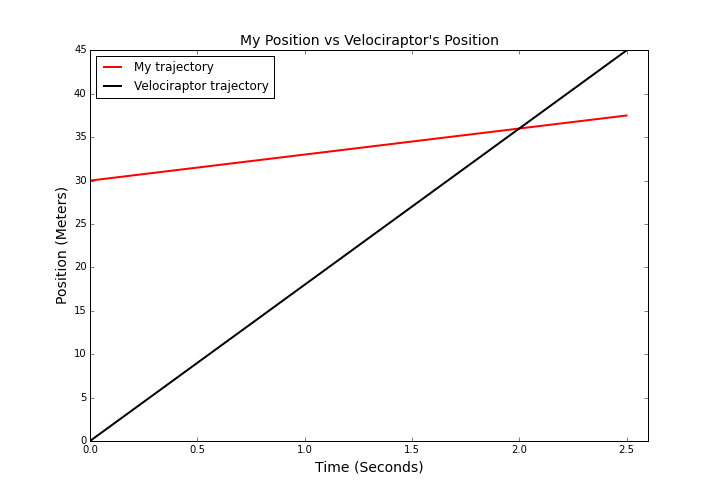
\includegraphics[width=0.5\textwidth]{humanvelociraptorpositionvstime.png}
    \caption{Python plot of a human and velociraptor's position as a function of time. \label{fig:siena}}
\end{figure}
%%%%%%%%%%%%%%%%%%%%%%%%%%%%%%%%%%%%%%%%%%%%%%%%%%%%%%%%%%%%%%%%%%%%%%%%%%%%%%%%
\end{document}
%%%%%%%%%%%%%%%%%%%%%%%%%%%%%%%%%%%%%%%%%%%%%%%%%%%%%%%%%%%%%%%%%%%%%%%%%%%%%%%%
